\chapter{Resultados}

Neste capítulo inicialmente será analisada as principais diferenças entre as implementações em Clojure e Haskell. Em seguida, será descrito em detalhes como foram realizados os experimentos para comparar as duas implementações em termos de desempenho e complexidade do código.

\section{Comparação das implementações}

O principal ponto de divergência entre as duas implementações está relacionado ao fato do modelo de STM de Clojure não prover o operador de bloqueio. Como em Haskell existe esse operador (a função \verb|retry|) todo compartilhamento de memória e sincronização das \emph{threads} pôde ser feito utilizando apenas memória transacional.

Em decorrência dessa limitação, alguns dos mecanismos utilizados na implementação em Haskell tiveram que ser reestruturados na implementação em Clojure. O principal exemplo dessa diferença é o modelo produtor-consumidor, descrito atenriormente, que foi bastante utilizado na solução proposta para compartilhar memória e sincronizar as \emph{threads}. Em Haskell, foram utilizados \emph{buffers} compartilhados entre as \emph{threads} para realizar essa tarefa. Esses \emph{buffers} foram contruídos utilizando \verb|TChan|s\footnote{http://hackage.haskell.org/packages/archive/stm/2.4.2/doc/html/Control-Concurrent-STM-TChan.html}, que internamente são modelados utilizando duas \verb|TVar|s. A principal função desses \emph{buffers} é, além de compartilhar memória entre as \emph{threads}, bloquear os consumidores que tentam realizar leitura quando o \emph{buffer} está vazio.

Em Clojure, a única maneira se simular exatamente o mesmo funcionamento do modelo produtor-consumidor utilizado em Haskell é através da classe \verb|LinkedBlockingQueue|\footnote{http://docs.oracle.com/javase/7/docs/api/java/util/concurrent/LinkedBlockingQueue.html} de Java ou semelhantes. Essa classe é implementa utilizando \emph{locks} (mais especificamente, \verb|ReentrantLock|\footnote{http://docs.oracle.com/javase/7/docs/api/java/util/concurrent/locks/ReentrantLock.html}) para garantir o bloqueio dos consumidores. A utilização dessa classe foi minimizada ao máximo com o objetivo utilizar na solução implementada em Clojure as construções que são providas diretamente pela linguagem. Dessa forma, apenas o \emph{buffer} utilizado para compartilhar os subíndices disponíveis entre as \emph{threads} de processamento e indexação foram modelos por meio da classe \verb|LinkedBlockingQueue|.

As demais utilizações do modelo produtor-consumidor foram representadas em Clojure como uma comunicação assíncrona por meio de notificações. Para isso foram utilizados os agentes, descritos na Seção 3.3. Os agentes provêem uma unidade de memória compartilhada que é atualizada através de ações assíncronas executadas em uma \emph{thread} separada. Além disso é possível registrar funções a um agente, conhecidas como \verb|watchers|\footnote{http://clojure.github.io/clojure/clojure.core-api.html\#clojure.core/add-watch}, que serão chamadas sempre que o valor do agente mudar (semelhante a um mecanismo de \emph{callbacks}). A comunicação com o \verb|Logger|, por exemplo, foi modelada dessa forma. Ao invés de manter uma \emph{thread} dedicada que fica bloqueada esperando novas mensagens serem adicionadas ao \emph{buffer}, um agente é utilizado para guardar as mensagens enviadas ao \verb|Logger|. Dessa forma, para enviar uma mensagem para o \verb|Logger|, a \emph{thread} remetente deve enviar uma ação de \emph{append} junto com mensagem em questão para um agente específico, que é executada assincronamente em outra \emph{thread} gerenciada pelo \emph{runtime} de Clojure. Depois, quando essa ação for executada, uma função específica que foi registrada como \verb|watcher| do agente do \verb|Logger| será responsável por processar a mensagem inserida e imprimí-la com a formatação correta para o usuário.

Outra divergência, indiretamente relacionada ao fato de Clojure não prover o operador de bloqueio, foi notada após o término das implementações. A quantidade de transações em memória que realizam mais de uma operação é consideravelmente reduzida na implementação em Clojure ao comparar-se à implementação em Haskell. Isso aconteceu porque a maioria das transações que tinham essa característica na implementação em Haskell estavam relacionadas ao \emph{buffer} compartilhado entre as \emph{threads}. 

\begin{listing}[h]
  \begin{minted}{haskell}
data Buffer a = Buffer (TChan a) (TVar Int) (TVar Bool)

newEmptyBuffer :: STM (Buffer a)
readBuffer :: Buffer a -> STM (Maybe a)
writeBuffer :: Buffer a -> a -> STM ()
enableFlag :: Buffer a -> STM ()
readFlag :: Buffer a -> STM Bool
  \end{minted}
  \caption{API do módulo Buffer da implementação em Haskell}
  \label{code:buffer-api}
\end{listing}

Para deixar essa relação mais clara, considere a API do módulo \verb|Buffer| mostrada no Código \ref{code:buffer-api}. Primeiro note que um \verb|Buffer| é representado através de um \verb|TChan|, que é o \emph{buffer} de fato, um \verb|TVar Int| que mantém a quantidade de elementos armazenados no momento e um \verb|TVar Bool| que é uma \emph{flag} indicando se a produção já terminou. Analizando a assinatura dos tipos das funções desse módulo, também é fácil de perceber que toda manipulação do \verb|Buffer| só pode ser feita dentro de uma transação. Como o \verb|Buffer| é representado como um tipo composto, e todos os valores que ele contém são variáveis transacionais, todas as operações desse módulo, por si só já executam mais de uma operação por transação. Por exemplo, sempre que um elemento é adicionado ao \emph{buffer}, além desse elemento ser adicionado ao \verb|TChan|, o contador também deve ser incrementado, caracterizando uma operação composta, já que outras \emph{threads} não devem ter acesso ao estado em que um elemento foi adicionado ao \emph{buffer} e o contador ainda não foi incrementado. Na utilização dessa API também é necessário utilizar composição de operações: quando a produção termina, geralmente, quando o produtor sabe que a produção acabou, ele executa uma transação que adiciona o último elemento ao \emph{buffer} e ao "mesmo tempo" chama a função \verb|enableFlag| para informar as \emph{threads} consumidoras que a produção terminou. Dessa forma, os consumidores conseguem ser informados quando suas execuções devem terminar.

De forma resumida, essas são as principais diferenças entre as duas implementações. Existem outros pontos de divergência mas que não são diretamente relacionados à maneira que o problema foi modelado e implementado mas sim com a diferença entre as linguagens que são diversas, desde o funcionamento do sistema de tipos até como as APIs fornecidas pelas bibliotecas padrão são projetadas.


\section{Experimentos}

Para analisar o desempenho das implementações em Clojure e Haskell foi utilizada uma base de documento composta de 60 livros de domínio público em lingua inglesa que foram obtidos por meio do projeto Gutenberg\footnote{http://www.gutenberg.org/}, totalizando 36 \emph{megabytes} de arquivos texto. Foram utilizadas também seis consultas com tamanhos distintos e ocorrências variadas na base de documentos. Os experimentos foram executados em uma máquina com processador Intel Core i7-3770 3.4GHz com 4 núcleos físicos e 8 \emph{gigabytes} de memória RAM rodando Linux. Para o ambiente Haskell foi utilizado o compilador GHC 7.6.2 junto com a \emph{flag} de compilação \verb|-O|. Já para o ambiente Clojure foi utilizado Clojure 1.5.1 com OpenJDK 7.u17.

Todo o código produzido neste trabalho é aberto e está disponível junto com o histórico de desenvolvimento no GitHub\footnote{https://github.com/luisgabriel/tsearch}\footnote{https://github.com/luisgabriel/tsearch-clj}.

\begin{figure}[h]
 \centering
 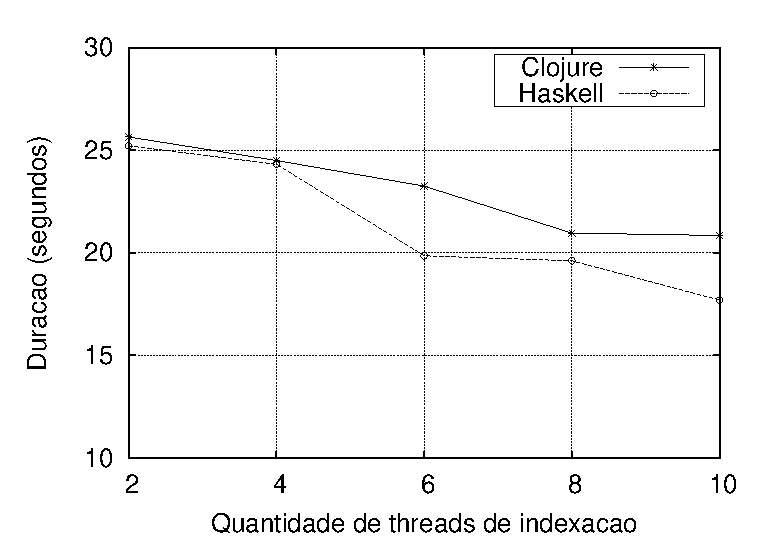
\includegraphics[scale=0.85]{imagens/clojure-haskell.eps}
 \caption{Gráfico do desempenho das versões paralelas em Clojure e Haskell}
 \label{fig:clj-hs-comp}
\end{figure}

A Figura \ref{fig:clj-hs-comp} mostra um gráfico onde o eixo horizontal representa a quantidade de \emph{threads} passada como argumento para o programa e o eixo vertical a duração em segundos da execução do programa. Cada ponto do gráfico representa a média do tempo de execução obtido a partir de 10 execuções consecutivas do programa calculado por meio do comando \verb|time| do Unix.

Como pode-se perceber, o desempenho de ambas as implementações foi bastante semelhante. As duas apresentaram melhora do desempenho total do sistema com o aumento do número de \emph{threads}. Porém, a melhoria de desempenho não foi grande se comparada ao aumento nos recursos de processamento disponíveis. 

\begin{figure}[h]
 \begin{minipage}{0.5\textwidth}
  \centering
  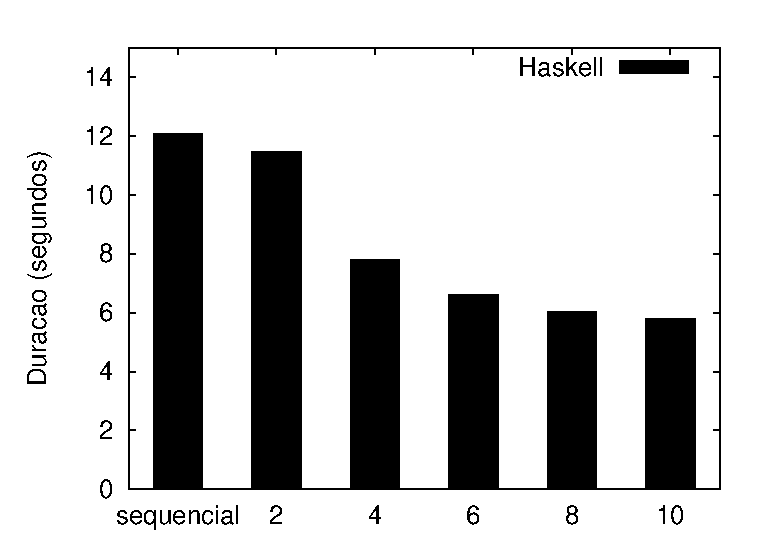
\includegraphics[scale=0.63]{imagens/haskell.eps}
 \end{minipage}
 \begin{minipage}{0.5\textwidth}
  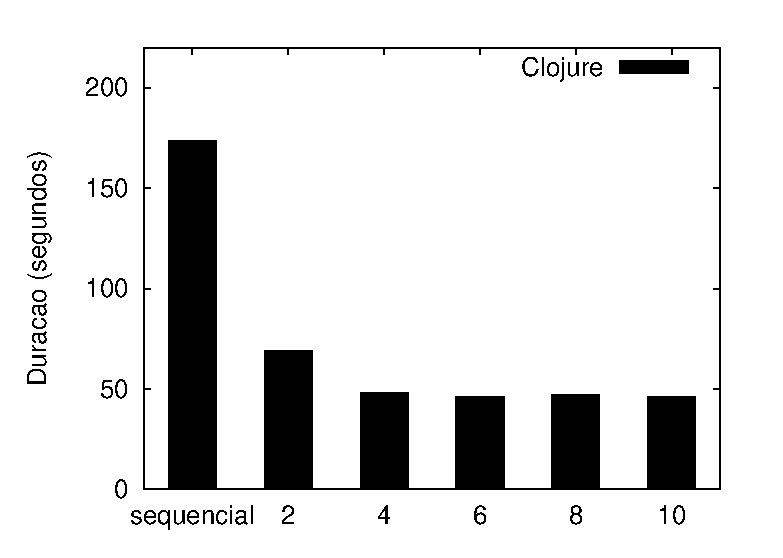
\includegraphics[scale=0.63]{imagens/clojure.eps}
 \end{minipage}
 \caption{Gráficos de comparação de desempenho entre das versões sequenciais e paralelas}
 \label{fig:clj-hs}
\end{figure}

Algumas características de cada implementação podem ter contribuído para que o aumento de desempenho não fosse tão alto. Na implementação em Haskell, por exemplo, utilizou-se memória transacional de forma excessiva, inclusive em cenários onde não haviam operações compostas. Dado que existe um \emph{overhead} relacionado à manutenção de \emph{logs} e sincronização das transações, é possível que esse fato tenha contribuído para degradar o desempenho total do sistema. Já na versão Clojure, pode-se citar a utilização de \emph{threads} do sistema operacional ao invés de \emph{green threads} como um fato que pode ter contribuído para a pequena melhora no desempenho do programa. Estudos subseqüentes precisarão analisar com mais profundidade os fatores que acarretaram no comportamento não-escalável dessas implementações.

\begin{figure}[h]
 \centering
 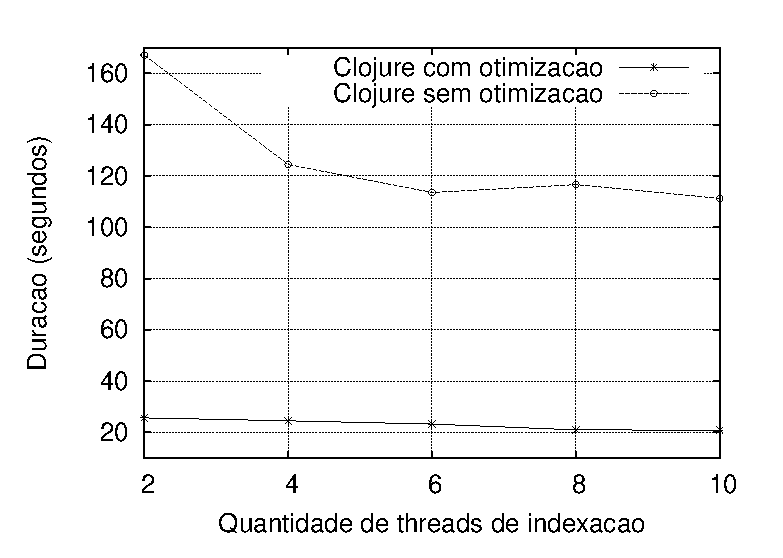
\includegraphics[scale=0.85]{imagens/clojure-opt.eps}
 \caption{Gráfico de comparação das versões em Clojure com e sem otimização}
 \label{fig:clj-opt}
\end{figure}

A Figura \ref{fig:clj-hs}, por sua vez, mostra os mesmos dados do gráfico anterior com a adição dos resultados obtidos da execução dos mesmos experimentos com as implementações sequenciais em cada linguagem. Com esses gráficos pode-se notar que o principal objetivo da paralelização do problema foi alcançado já que a versão paralela, em todas as configurações testadas, conseguiu ter desempenho melhor que a versão sequencial.

Também é importante observar que foi necessário aplicar, após finalização da implementação, algumas otimizações ao código em Clojure para que fosse possível atingir o desempenho apresentado nas Figuras \ref{fig:clj-hs-comp} e \ref{fig:clj-hs}. Como pode-se verificar na Figura \ref{fig:clj-opt}, a diferença de desempenho com e sem otimização é muito grande. A principal causa dessa diferença está atrelada ao uso de reflexão por parte do compilador de Clojure para realizar chamadas de métodos Java. Para que o código desenvolvido nesse trabalho tivesse um desempenho aceitável, foi necessário utilizar anotações de tipos em pontos do código onde métodos Java eram chamados diretamente. Esse resultado é importante pois mostra que, apesar das vantagem impostas pela tipagem dinâmica de Clojure, o desempenho da linguagem é fortemente afetado pela presença de informação de tipo em tempo de compilação

\begin{figure}[!h]
 \begin{minipage}{0.5\textwidth}
  \centering
  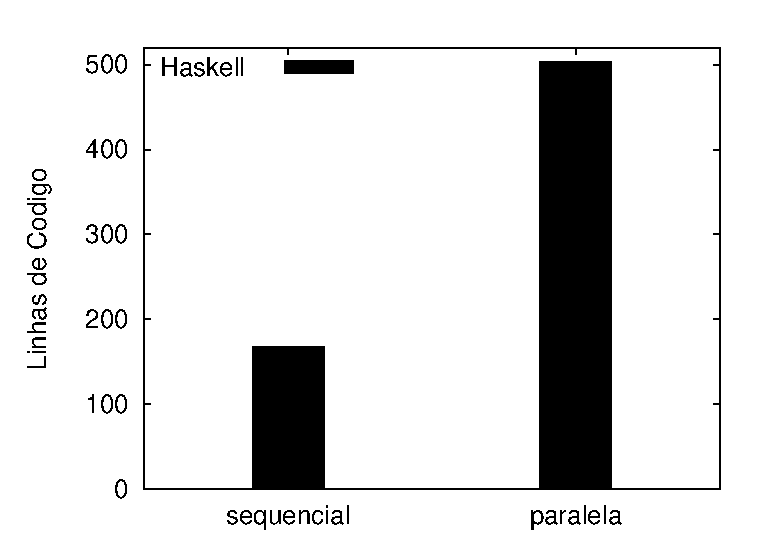
\includegraphics[scale=0.63]{imagens/loc-haskell.eps}
 \end{minipage}
 \begin{minipage}{0.5\textwidth}
  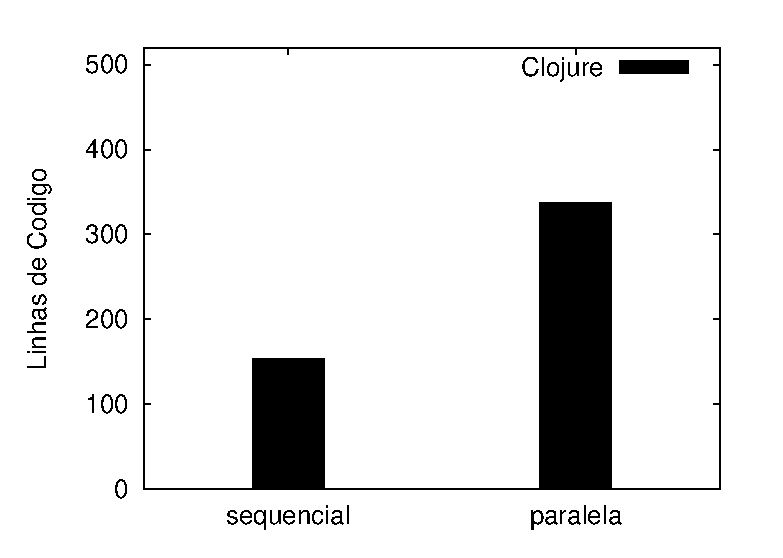
\includegraphics[scale=0.63]{imagens/loc-clojure.eps}
 \end{minipage}
 \caption{Gráficos de comparação da quantidade de linhas de código}
 \label{fig:clj-hs-loc}
\end{figure}

Por fim, a Figura \ref{fig:clj-hs-loc} mostra o comparativo entre a quantidade de linhas de código total de todas as implementações. Como pode-se perceber, a paralelização implicou em um aumento considerável na quantidade de linhas de código dos projetos. No caso de Clojure, foi um aumento de aproximadamente 120\%, enquanto em Haskell foi um aumento de 200\%. Esse resultado mostra que, de fato, paralelizar um programa implica no aumento da complexidade da solução. Em um ambiente industrial, se faz necessário uma análise mais minuciosa para entender a relação de custo-benefício de se escrever sistemas concorrentes, pois, dependendo do cenário, melhorar o desempenho de um sistema em torno de 40\% ao custo de duplicar ou triplicar a base de código pode ser inaceitável.